\documentclass[onecolumn, draftclsnofoot,10pt, compsoc]{IEEEtran}
\usepackage{graphicx}
\usepackage{url}
\usepackage{setspace}

\usepackage{geometry}
\geometry{textheight=9.5in, textwidth=7in}

% 1. Fill in these details
\def \CapstoneTeamName{		    The Apolloers}
\def \CapstoneTeamNumber{		49}
\def \GroupMemberOne{			Jonathan Ropp}
\def \GroupMemberTwo{			Shannon Sandy}
\def \GroupMemberThree{			Dean Akin}
\def \CapstoneProjectName{		Apollo 11 3D Animation}
\def \CapstoneSponsorCompany{	OMSI}
\def \CapstoneSponsorPersona{	Jim Todd}
\def \CapstoneSponsorPersonb{	Mike Bailey}

% 2. Uncomment the appropriate line below so that the document type works
\def \DocType{		
                %Problem Statement
				Requirements Document
				%Technology Review
				%Design Document
				%Progress Report
				}
			
\newcommand{\NameSigPair}[1]{\par
\makebox[2.75in][r]{#1} \hfil 	\makebox[3.25in]{\makebox[2.25in]{\hrulefill} \hfill		\makebox[.75in]{\hrulefill}}
\par\vspace{-12pt} \textit{\tiny\noindent
\makebox[2.75in]{} \hfil		\makebox[3.25in]{\makebox[2.25in][r]{Signature} \hfill	\makebox[.75in][r]{Date}}}}
% 3. If the document is not to be signed, uncomment the RENEWcommand below
\renewcommand{\NameSigPair}[1]{#1}

%%%%%%%%%%%%%%%%%%%%%%%%%%%%%%%%%%%%%%%
\begin{document}
\begin{titlepage}
    \pagenumbering{gobble}
    \begin{singlespace}
        \hfill 
        % 4. If you have a logo, use this includegraphics command to put it on the coversheet.
        
\includegraphics[height=4cm]{OSU_horizontal_2C_O_over_B.eps}   
        \par\vspace{.2in}
        \centering
        \scshape{
            \huge CS Capstone \DocType \par
            {\large\today}\par
            \vspace{.5in}
            \textbf{\Huge\CapstoneProjectName}\par
            \vfill
            {\large Prepared for}\par
            \Huge \CapstoneSponsorCompany\par
            \vspace{5pt}
            {\Large\NameSigPair{\CapstoneSponsorPersona}\par}
            {\Large\NameSigPair{\CapstoneSponsorPersonb}\par}
            {\large Prepared by }\par
            Group\CapstoneTeamNumber\par
            % 5. comment out the line below this one if you do not wish to name your team
            \CapstoneTeamName\par 
            \vspace{5pt}
            {\Large
                \NameSigPair{\GroupMemberOne}\par
                \NameSigPair{\GroupMemberTwo}\par
                \NameSigPair{\GroupMemberThree}\par
            }
            \vspace{20pt}
        }
        \begin{abstract}
        % 6. Fill in your abstract    
        	Our group, The Apolloers, is working with Mike Bailey to create a 3D animation about the Apollo 11 Moon Landing. This animation will be put on display in OMSI during the Summer of 2019 for the 50th anniversary of the Apollo 11 mission. All parts of the mission will be included, from Earth Launch to Earth landing, and all sections in between. This document breaks the project into requirements that we will use to guide our project through the development process. 
        \end{abstract}     
    \end{singlespace}
\end{titlepage}
\newpage
\pagenumbering{arabic}
\tableofcontents
% 7. uncomment this (if applicable). Consider adding a page break.
%\listoffigures
%\listoftables
\clearpage

% 8. now you write!
\section{Introduction}
Our group will be recreating the Apollo 11 mission in a 25-minute video using 3D graphics. This project is for the Oregon Museum of Science and Industry to display in their planetarium for the 50th anniversary of the Apollo 11 mission. This document contains the requirements for this project that our group and clients, Jim Todd and Mike Bailey, have agreed upon. These requirements act as a definitive list of features that our project will need to implement in order for it to be considered complete. 
    \subsection{Purpose}
    The purpose of this project is to educate the general public about the Apollo 11 mission as well as to commemorate the mission's 50th anniversary. Our goal is to create the video so that the audience at OMSI will appreciate the complexity of the mission while also being entertained. 
    \subsection{Scope}
    This project will be a 25 minute video whose target audience are the people attending the planetarium at OMSI. This includes school children on a field trip, people interested in space travel, and people who are attending the planetarium to be entertained. Since the planetarium at OMSI has a large audience of diverse people, the Apollo 11 recreation will need to be accessible, entertaining, as well as realistic in order to educate the audience without boring them.
    \subsection{Overview}
    For the video of the Apollo 11 to be considered complete the following features will need to be implemented: textured 3D objects, a variety of camera positions for the viewer, the flight path of Apollo 11, docking of the modules, physics, and audio files and transcriptions. This is a general overview of the requirements for this project. The System Requirements section will go into more detail explaining  
    \subsection{Definitions}
\begin{tabular} {|l|p{13.5cm}|}
    \hline
    Term & definition \\ \hline
    API & An Application Programming Interface is a set of protocols and tools that are used to build a software application. Essentially the `building blocks' that a programmer uses to build an application.  \\ \hline
    Apollo 11 Mission & A spaceflight operated by NASA to land the first humans on the Moon, launched July 16th, 1969.  \\ \hline
    NASA & The National Aeronautics and Space Administration is a federal agency that focuses on research and development related to air and space.	\\ \hline
    OMSI & The Oregon Museum of Science and Industry, located in Portland, Oregon	\\ \hline
    OpenGL & An open-source graphics library API that is used to interact with graphics hardware to design 3D renderings.	\\ \hline
    SDK & A Software Development Kit is a set of tools that program developers use to write programs for an application. \\ \hline

\end{tabular}
\section{Specific Requirements}
    \subsection{External Interfaces}
    At minimum, the animation will need to be viewed on some sort of computer display. Ideally, we will be able to gain access to OMSI's projector SDK so that we can display the animation in OMSI's planetarium through 10 projectors. There will also be audio alongside the animation, such as the sounds of the boosters, mission communications, and possibly captions.
    \subsection{Functions}
    The 3D animation of the Apollo 11 Mission will include the entire flight path (launch to orbit, orbit to trans-lunar injection, to moon, to lunar orbit, to landing, to re-launch, to lunar orbit, to trans-Earth injection, to Earth, to splashdown). 3D objects will include the Earth, Moon, Lunar Module \textit{Eagle}, Saturn 5 rocket, Command Module, and others as we see fit. All of these sections will be smoothly animated together and be as scientifically accurate as possible.
    \subsection{Usability Requirements}
    Users will be able to view the animation from arbitrary viewpoints. This will be controlled by a computer mouse and keyboard, and be designed in such a way that any user, even without vast knowlege of computers, would be able to fully intereact with the animation. There will also be static viewpoints placed inside the command module that users can swap to using the keyboard. 
    \subsection{Performance Requirements}
    The animation will need to run at a steady frame rate throughout the whole mission to avoid breaking immersion. Also, there cannot be any errors when running the program; it will need to be robust enough to run without interuption even in edge-case environments.
\section{Verification}
    \subsection{External Interfaces}
    Minimally, we can make sure that we can view the animation from a computer display. Then, if we gain access to the projector SDK, we can attempt to view the animation in OMSI's planetarium and make sure the animation scales to the correct size. Also, we need to make sure the audio sounds good from a computer station, but if we present in the planetarium, we will need to make sure the audience is treated to the best audio the planetarium can provide. 
    \subsection{Functions}
    We will make sure to include all parts of the flight path in the animation and these scenes need to transition from one to the other without any noticeable change. We will have 3D objects for all notable objects in the animation (Earth, Moon, Saturn 5 Rocket, etc.). Ideally, we will use physics for all movement, but a reasonable goal would be to have at least half the movement be based on real physics and used idealized motion for the rest.
    \subsection{Usability Requirements}
    Allow a user from outside of our project group take control of the animation and make sure that they system is user-friendly. They 
    should be able to fully operate the program with minimal instruction from our group. User testing may be organized later in the development cycle to ensure that a wide variety of users from different backgrounds are not struggling to interact with the animation. 
    \subsection{Performance Requirements}
    On a suitable, mid-range computer, the animation should be able to run and keep a steady frame rate even when given extreme values for input. Ideally, the animation will run at 60 frames per second with little variation, but even more important than the frames per second is that the animation is not `choppy' and is easy to watch.

\section{Gantt Chart}

\begin{figure}[!htb]
    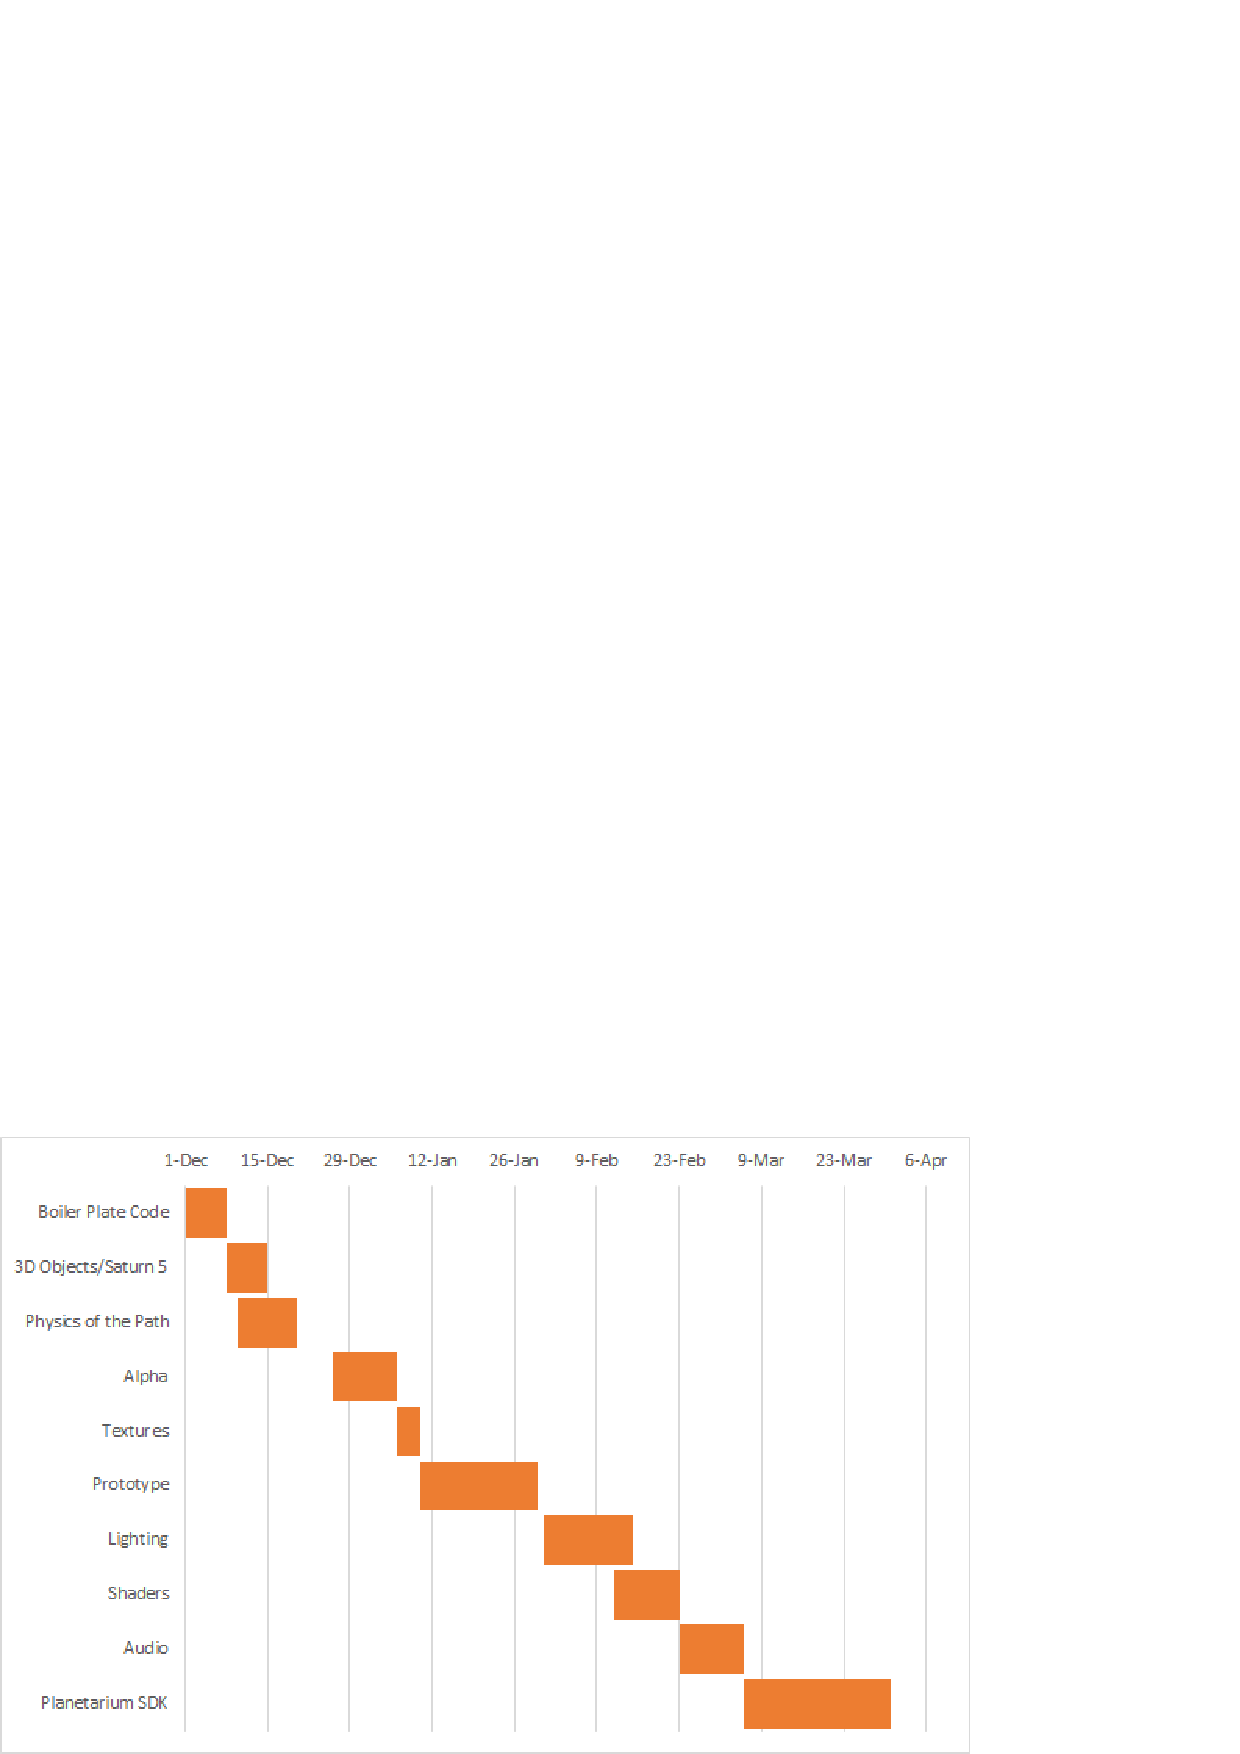
\includegraphics[width=\linewidth]{Gantt.PNG}
    \caption{Gantt chart of proposed timeline}
    \label{fig:Gantt Chart}
\end{figure}

\section{Appendix}
Since this document was first drafted, the requirements for our project have changed. On January 3rd, our team and Mike Bailey drove to OMSI to meet with our client, Jim Todd, for the first time. During our meeting, Jim Todd provided our team with more refined requirements for our video. The most significant change was that Jim Todd wanted our animation to recreate the aspects Apollo 11 mission that took place on the lunar surface. Instead of animating the launch, flight to the moon, and flight back to Earth, our team will now include historic audio/video to provide context to the Apollo 11 mission. 

Our team will also include a default video that can be paused and restarted whenever the audience wishes to change viewpoints. The video will be from the perspective of an astronaut as he leaves the lunar module, travels the lunar surface, plants the American flag, and finally board the lunar module for lunar launch. Changing viewpoints during the default video will pause the animation and the user will be able to press a key on the keyboard to continue the video.

Our video will now be 10-15 minutes long instead of 20 minutes. This change was made because each planetarium show is 20 minutes long and our team wanted to allow the audience time to ask any questions about the Apollo 11 mission during the show.

\end{document}
